\subsection{Earlier admission windows and historical search}\label{app:record-windows}

The main text selects four views of admission decisions and operating
activity. The additional figures here retain the earlier windows and
alternative summaries, with their original captions and observations.
\Cref{fig:fw-validation} covers the earlier admission prefix;
\cref{fig:fw-trainval,fig:fw-telemetry} resolve a smaller set of retained
summaries. Gaps between windows are not filled or treated as observations.

\begin{figure}[t]
  \centering
  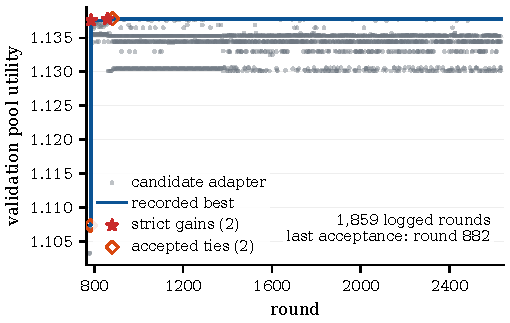
\includegraphics[width=\linewidth]{figures/fig_fw_live_validation.pdf}
  \caption{\textbf{Adapter validation and admissions.} The \num{1889}-round window,
  775--2663: grey candidate utility, blue recorded best; stars mark strict gains,
  hollow diamonds accepted ties. \Cref{app:latest-admissions} extends through round 2837.}
  \label{fig:fw-validation}
\end{figure}

\begin{figure*}[t]
  \centering
  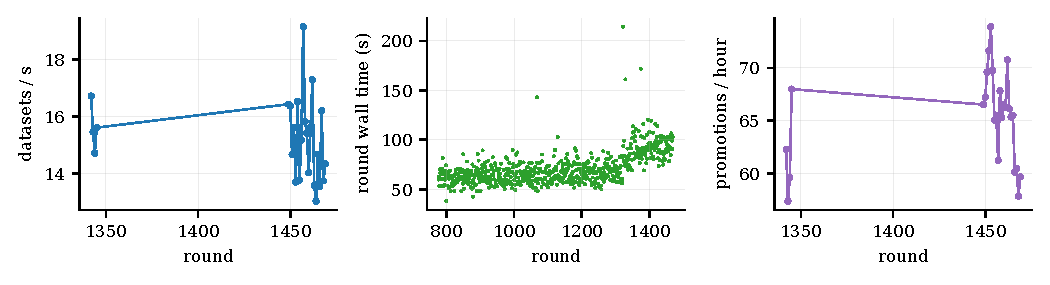
\includegraphics[width=\linewidth]{figures/fig_fw_telemetry.pdf}
  \caption{\textbf{Operating measurements from earlier retained windows.}
  Left/right: 25 summaries spanning rounds 1342--1469. Middle: intervals
  between logged admission timestamps within 775--1469. Green: positive
  intervals under 600\,s. Blue squares: 25 logged round wall times. Left:
  distinct training contexts divided by completed-round wall time. Right:
  strict improvements to training-program incumbents per hour, using accumulated
  wall time over up to twenty completed rounds in the reporting process,
  including qualification waits. Program events and adapter admissions count
  different outcomes. These are earlier operating windows within
  \cref{fig:fw-validation}, not one-proposal deployment accuracy or cost.}
  \label{fig:fw-telemetry}
\end{figure*}

\begin{figure}[t]
  \centering
  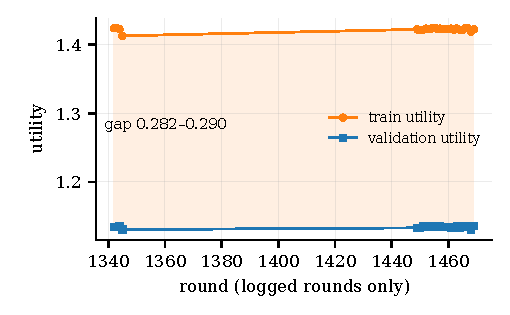
\includegraphics[width=\linewidth]{figures/fig_fw_train_val.pdf}
  \caption{\textbf{Train and validation aggregates on retained summaries.}
  The 25 summaries span rounds 1342--1469; a broken axis separates the
  observed blocks. Intervening summaries are not retained; the utility
  gap covers only these 25 summaries.}
  \label{fig:fw-trainval}
\end{figure}






Lower predicted cost is preferred. Logged utility averages the selected
programs' recorded outcomes; it is not the adapter's cost prediction.
For new proposals, the caller uses predicted costs and an exploration
setting to select programs for exact evaluation. The referee still decides
validity and improvement. Logging an evaluation does not itself add the
program to the adapter's training pool.

The admission prefix covers \num{1889} consecutive rounds, 775--2663.
Four rows are marked accepted: two strict best increases and two ties.
Within this 775--2663 window, the recorded best remains 1.1378. After the tie
at round 882, all \num{1781} remaining rounds in that window are rejected (\cref{fig:fw-validation}; see \cref{app:acceptance-over-rounds} for the isolated recorded-best trajectory and cumulative acceptance rate).
Comparisons across harnesses need matched data, normalization and scoring
protocols.

The older detailed summaries cover only 25 of those rounds. In that subset,
training utility exceeds validation utility by 0.282--0.290
(\cref{fig:fw-trainval}). This is a difference between reported aggregates
on separate training and validation contexts; it does not isolate a cause
or establish behavior in the missing summaries. The late validation plateau
is evidence to explain, rather than proof of useful transfer. Encoder
integrity and parameter updates require their own receipts; the plotted
utility tables do not establish either.
\Cref{fig:fw-telemetry} shows the loop's operating measurements from the earlier
retained window.

\begin{figure}[t]
  \centering
  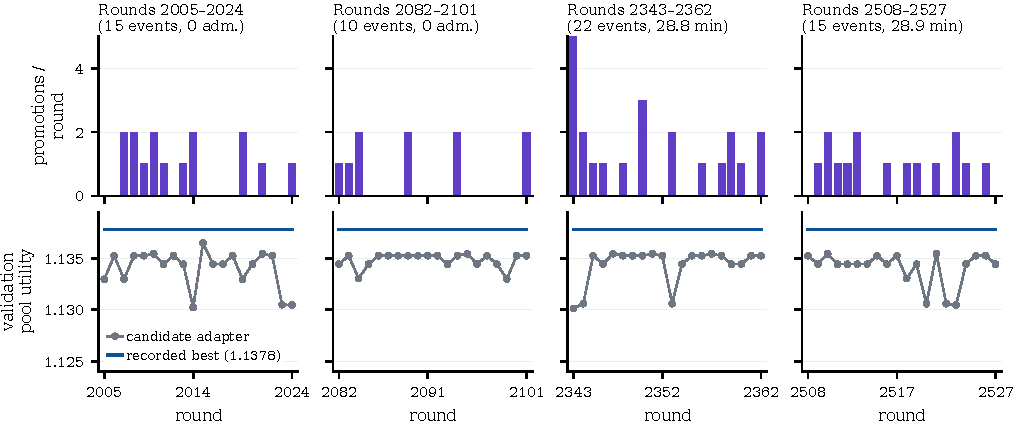
\includegraphics[width=\linewidth]{figures/fig_fw_recent_development.pdf}
  \caption{\textbf{Program promotions and adapter utility in an additional window.}
  Top: cumulative logged strict improvements to training-program incumbents,
  reset to zero at the start of this window. Bottom: candidate adapter
  validation utility and the recorded best. Both panels use the same 20
  summaries from rounds 2005--2024. These are development measurements; neither
  the event count nor the utility curve establishes first-proposal improvement.}
  \label{fig:fw-recent-development}
\end{figure}

\begin{figure*}[t]
  \centering
  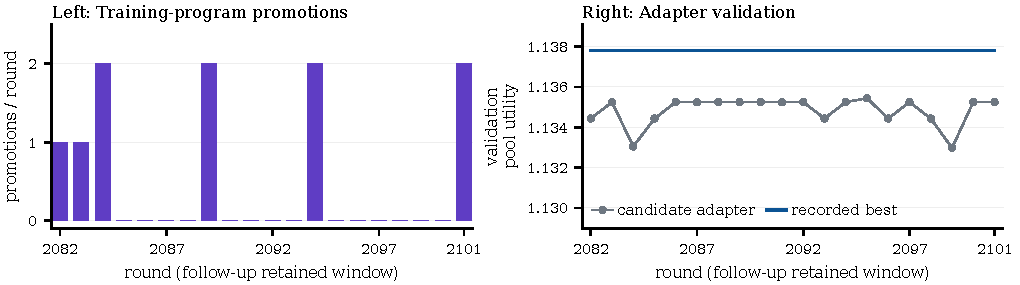
\includegraphics[width=\linewidth]{figures/fig_fw_followup_development.pdf}
  \caption{\textbf{Program events and adapter validation in a follow-up window.}
  Left: journaled strict training-program incumbent improvements per round.
  Right: candidate adapter validation pool utility and the recorded best.
  Both panels cover the same 20 consecutive summary rounds, 2082--2101. The summaries
  mark no adapter admission. Independent first-proposal and transfer tests
  remain required.}
  \label{fig:fw-followup-development}
\end{figure*}

The shorter retained windows give more detailed operating views. Rounds
2005--2024 appear in \cref{fig:fw-recent-development}, with cumulative
journaled strict program promotions counted from zero for that window.
The adapter panel separates candidate validation utility from the recorded
best. Rounds 2082--2101 follow in \cref{fig:fw-followup-development} (\cref{app:flywheel-telemetry}).

\begin{figure}[t]
  \centering
  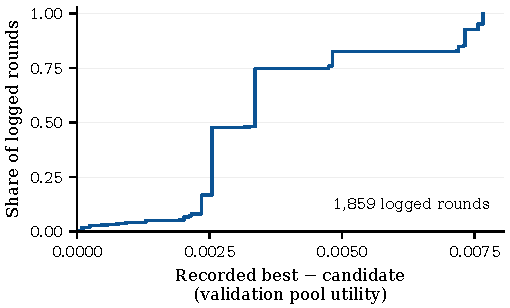
\includegraphics[width=\linewidth]{figures/fig_fw_live_shortfall.pdf}
  \caption{\textbf{Candidate gaps to the recorded best.} Cumulative share
  of the same \num{1889} admission rounds as \cref{fig:fw-validation}, against
  recorded best minus candidate validation utility. The best is logged
  after admission, so zero includes strict gains and ties. Repeated
  adaptive rounds are not independent trials.}
  \label{fig:fw-admission-shortfall}
\end{figure}

For the adapter record in \cref{fig:fw-validation},
\cref{fig:fw-admission-shortfall} summarizes candidate gaps to each round's
recorded best. Each retained round contributes once; the curve does not
count independent tasks or distinct programs.

\FloatBarrier
\begin{figure*}[t]
  \centering
  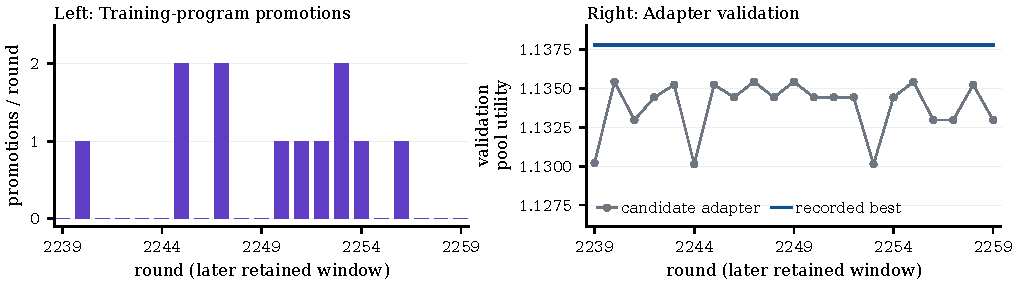
\includegraphics[width=\linewidth]{figures/fig_fw_later_development.pdf}
  \caption{\textbf{Continued program events and adapter validation.}
  Left: journaled strict training-program incumbent improvements per round.
  Right: candidate adapter validation pool utility and the recorded best.
  Both panels cover all 20 consecutive rounds, 2343--2362, in this retained summary
  window. The summaries mark no adapter admission. Independent
  first-proposal comparisons remain required.}
  \label{fig:fw-later-development}
\end{figure*}

The retained window at rounds 2343--2362 appears in
\cref{fig:fw-later-development} (\cref{app:flywheel-telemetry}). It records 22 strict training-program
improvements and no adapter admission. The logged best remains 1.1378,
labeled round 882 in these records. The 20 completed rounds total \num{1730.1}\,s of logged wall time: 41.6 rounds and 45.8 program promotions per
hour, including qualification waits. These program-event rates apply to
2343--2362, not all admission rounds through 2663 or one-proposal deployment.

\Cref{app:development-time} plots rounds 2343--2362 against accumulated
completed-round time. \Cref{app:event-counts} groups the three earlier
retained windows by training-program event count. Rounds 2508--2527 and
their work and event rates follow in
\cref{app:subsequent-window,app:subsequent-rates}.

\begin{figure}[t]
  \centering
  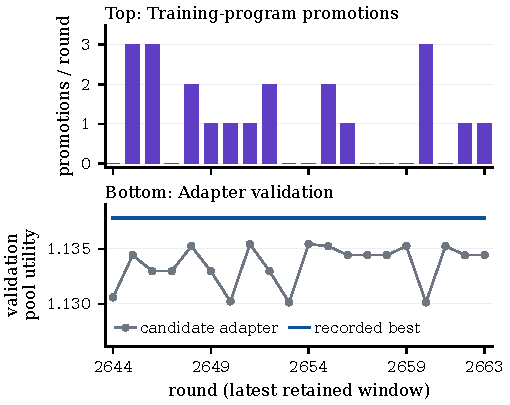
\includegraphics[width=\linewidth]{figures/fig_fw_live_development.pdf}
  \caption{\textbf{Program-incumbent events and validation summaries.}
  Top: logged strict improvements to training-program incumbents per round.
  Bottom: candidate adapter validation pool utility. Both panels cover the
  same 20 consecutive rounds, 2644--2663. These are development measurements;
  independent first-proposal comparisons remain required.}
  \label{fig:fw-program-promotions}
\end{figure}

The window at rounds 2644--2663 appears in
\cref{fig:fw-program-promotions}, with a per-hour view in \cref{fig:fw-promotions-per-hour} (\cref{app:promotions-per-hour}). It records 21 strict program promotions
and no adapter admission. The two panels align the program-event counts
with candidate validation utility for each round; the journal supplies
no confidence interval for those incumbent improvements.
The later rounds 2696--2715 appear in \cref{app:round-throughput}.

The main-text admission prefix through round 2837 appears in
\cref{app:latest-admissions,fig:fw-latest-admissions}. It extends the earlier
window without changing its observations; accepted ties remain distinct
from strict increases in retained-best utility.

\FloatBarrier
\begin{figure}[t]
  \centering
  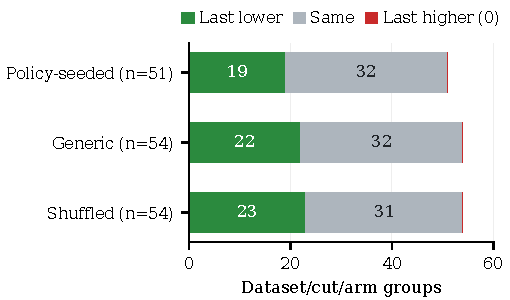
\includegraphics[width=\linewidth]{figures/fig_fw_target_progress.pdf}
  \caption{\textbf{Historical GP target progress.} First-to-last reported
  best development RMSE at \num{1000} evaluations per search, grouped by search
  arm. Lower is better; unchanged scores are included. The arms shared
  incumbent and teacher seeds, and elapsed time varied. These counts do
  not measure independent discoveries or a learned-policy advantage.}
  \label{fig:fw-target-progress}
\end{figure}

Historical GP target scores provide a separate view in
\cref{fig:fw-target-progress}. The 159 repeated dataset/cut/arm groups cover
55 distinct dataset/cut pairs; the 64 groups with lower final scores cover
23 pairs. Shared incumbent and teacher seeds make the arms dependent.
These retained development outcomes do not establish that learning improved
the proposal policy.

\begin{figure*}[t]
  \centering
  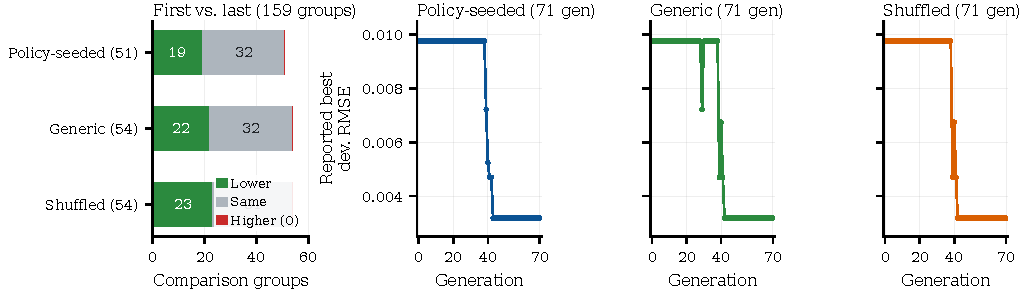
\includegraphics[width=\linewidth]{figures/fig_fw_target_history.pdf}
  \caption{\textbf{Post-hoc GP target trajectory.} All 71 generations per
  arm for one historical dataset/cut, at \num{1000} evaluations per search.
  RMSE is in historical evaluator units; lower is better. The arms shared
  incumbent and teacher seeds, and elapsed time varied. This selected
  development example does not establish a learned-policy advantage.}
  \label{fig:fw-target-history}
\end{figure*}

\Cref{fig:fw-target-history} follows one historical dataset/cut, chosen
after inspection for the largest policy-seeded relative improvement in
the preceding comparison set. Every reported generation is shown, without
applying a cumulative minimum. All three arms finish at the same value;
the policy-seeded arm first records it one generation after the controls.
Shared seeds prevent treating their matching outcomes as independent discoveries.
